\PassOptionsToPackage{dvipsnames,table}{xcolor}
\documentclass[10pt]{beamer}
\usepackage{Cours}

\begin{document}

\input{\detokenize{/home/fenarius/Travail/Cours/NSITerminale/docs/commun/MacrosCours.tex}}
\setcounter{numchap}{15}

\pythonmode

\newcommand{\SC}{\cnum Sécurisation des communications}

\pythonmode

\begin{frame}
	\mframe{\SC}
	\begin{block}{Vocabulaire}
		\begin{itemize}
			\item<1-> La \textcolor{blue}{cryptographie} est l'étude des méthodes permet de sécuriser une communication.
			\item<2-> Le \textcolor{blue}{chiffrement} d'un message est sa transformation en un une suite de caractère incompréhensible (dit \textit{texte chiffré}).
			\item<3-> Le chiffrement s'effectue via un algorithme nécessitant un paramètre appelé \textcolor{blue}{clé de chiffrement}. Et de même le déchiffrement nécessite une \textcolor{blue}{clé de déchiffrement}
			\item<4-> Lorsque la connaissance de ces deux clés doit rester secrète on dit qu'il s'agit d'un \textcolor{blue}{chiffrement symétrique}.
			\item<5-> Lorsque la clé de chiffrement peut être connu de tous (on parle alors de \textcolor{blue}{clé public}) et que seul la clé de déchiffrement reste secrète (on parle alors de \textcolor{blue}{clé privé}), on dit qu'il s'agit d'un \textcolor{blue}{chiffrement asymétrique}.
		\end{itemize}
	\end{block}
\end{frame}

\begin{frame}
	\mframe{\SC}
	\begin{block}{Représentation du chiffrement symétrique}
		\begin{center}
		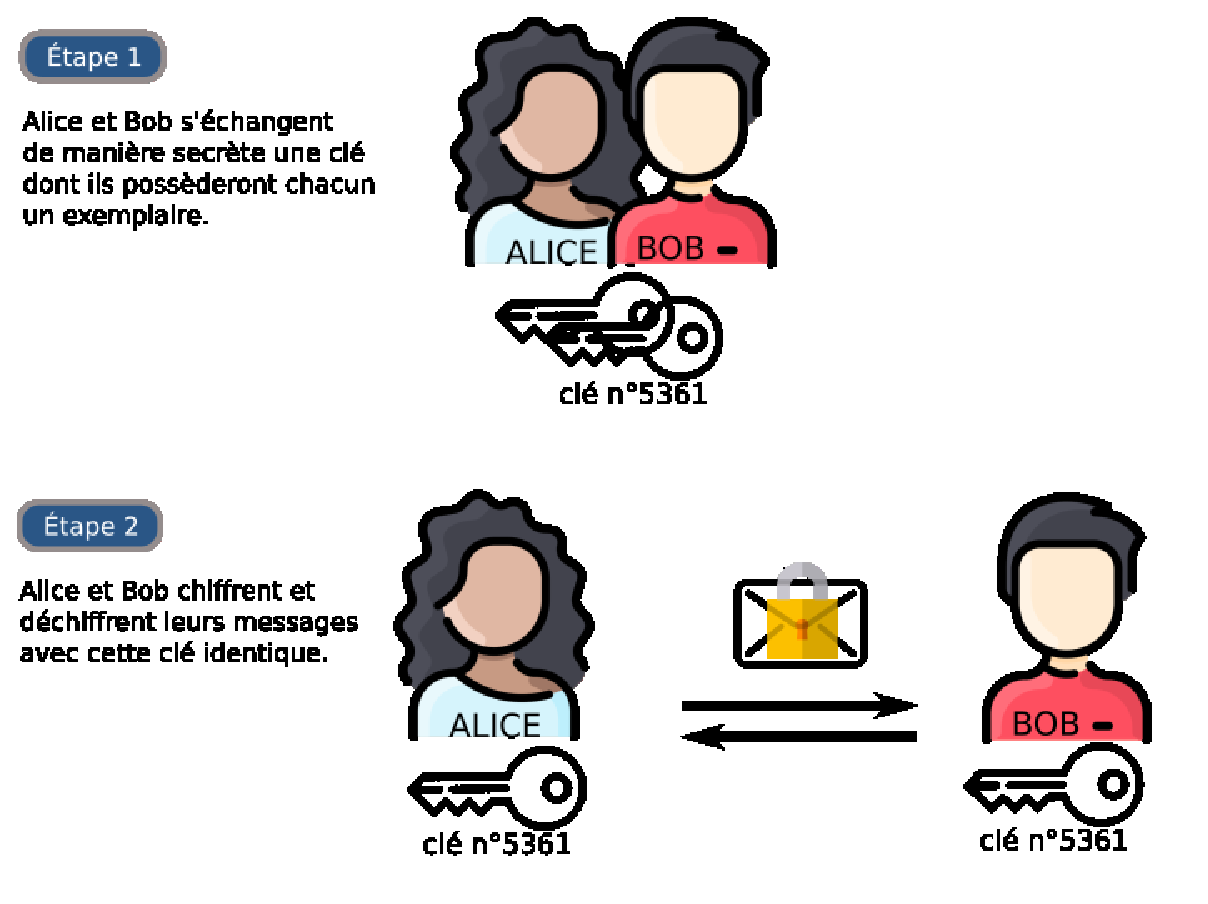
\includegraphics[height=160px]{sym.eps}
		\end{center}
	\end{block}
\end{frame}

\begin{frame}
	\mframe{\SC}
	\begin{block}{Représentation du chiffrement asymétrique}
		\begin{center}
		\includegraphics[height=160px]{asym.eps}
		\end{center}
	\end{block}
\end{frame}


\begin{frame}
	\mframe{\SC}
	\begin{exampleblock}{Exemples}
		\begin{enumerate}
		\item<1-> Le code de César est l'un des premiers exemples historique :
		\begin{itemize}
			\item<2-> La clé de chiffrement est un entier note $C$, par exemple 3.
			\item<3-> L'algorithme de chiffrement consiste alors à décaler chaque lettre de $C$ emplacements à droite dans l'alphabet. Avec une clé de 3, le message "NSI", se transforme  en "QVL".
			\item<4-> Pour déchiffrer on décale de $C$ emplacements à gauche.
			\item<5-> La connaissance des deux clés doit rester secrète, c'est donc un chiffrement symétrique.
		\end{itemize}
		\item<6-> Parmi les méthodes modernes (et bien plus robustes) de chiffrement symétrique, on peut citer : \textcolor{blue}{AES (Advanced Encryption Standard)} ou encore \textcolor{blue}{Chacha20}.
		\item<7-> L'exemple classique de chiffrement asymétrique est \textcolor{blue}{RSA} (voir activité.)
	\end{enumerate}
	\end{exampleblock}
\end{frame}


\begin{frame}
	\mframe{\SC}
	\begin{block}{Avantages et inconvénients des deux méthodes}
		\begin{itemize}
			\item<1-> Un chiffrement symétrique est souvent rapide et donc adapté au transfert d'un volume important d'informations.
			\item<2-> Un chiffrement symétrique peut-être très sûr (voire inviolable).\\
					\onslide<3->{\textcolor{OliveGreen}{\small Par exemple, un chiffrement {\sc xor} utilisant un masque aussi long que le message est inviolable}}
			\item<3-> L'inconvénient est que puisque le canal de transmission n'est pas sûr, les deux interlocuteurs doivent convenir \textcolor{blue}{au préalable} d'une clé de chiffrement.
			\item<4-> Dans un chiffrement asymétrique par contre, la clé de chiffrement peut être connue de tous car elle ne permet pas de déchiffrer. Elle peut donc être rendue publique sans mettre en danger la sécurité de la communication.
			\item<5-> Par contre, un chiffrement asymétrique peut être gourmand en ressource et donc non adapté à un volume important d'informations.
		\end{itemize}
	\end{block}
\end{frame}

\begin{frame}
	\mframe{\SC}
	\begin{block}{Protocole {\sc https}}
		Le protocole {\sc https} qui permet de sécuriser les transmissions est un exemple d'utilisation conjointe des deux méthodes : asymétrique et symétrique.
		\begin{center}
			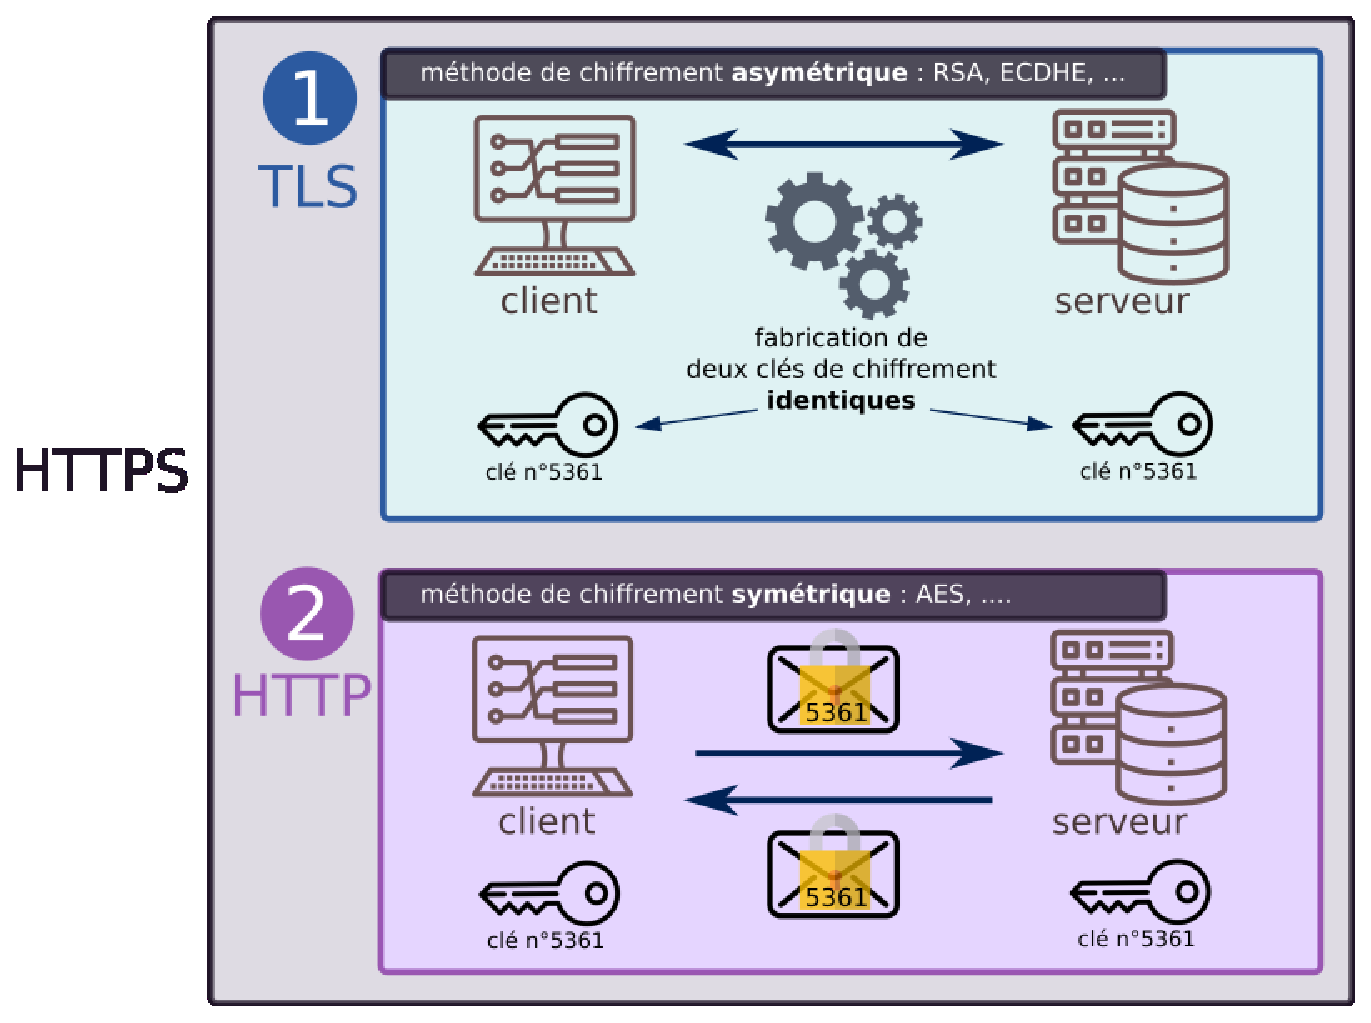
\includegraphics[height=160px]{https.eps}
		\end{center}
	\end{block}
\end{frame}

\begin{frame}
	\mframe{\SC}
	\begin{block}{Autorité de certification}
		D'autre part, afin d'éviter une attaque du type \textit{homme du milieu} une autorité extérieure garanti l'identité du serveur.
		\begin{center}
			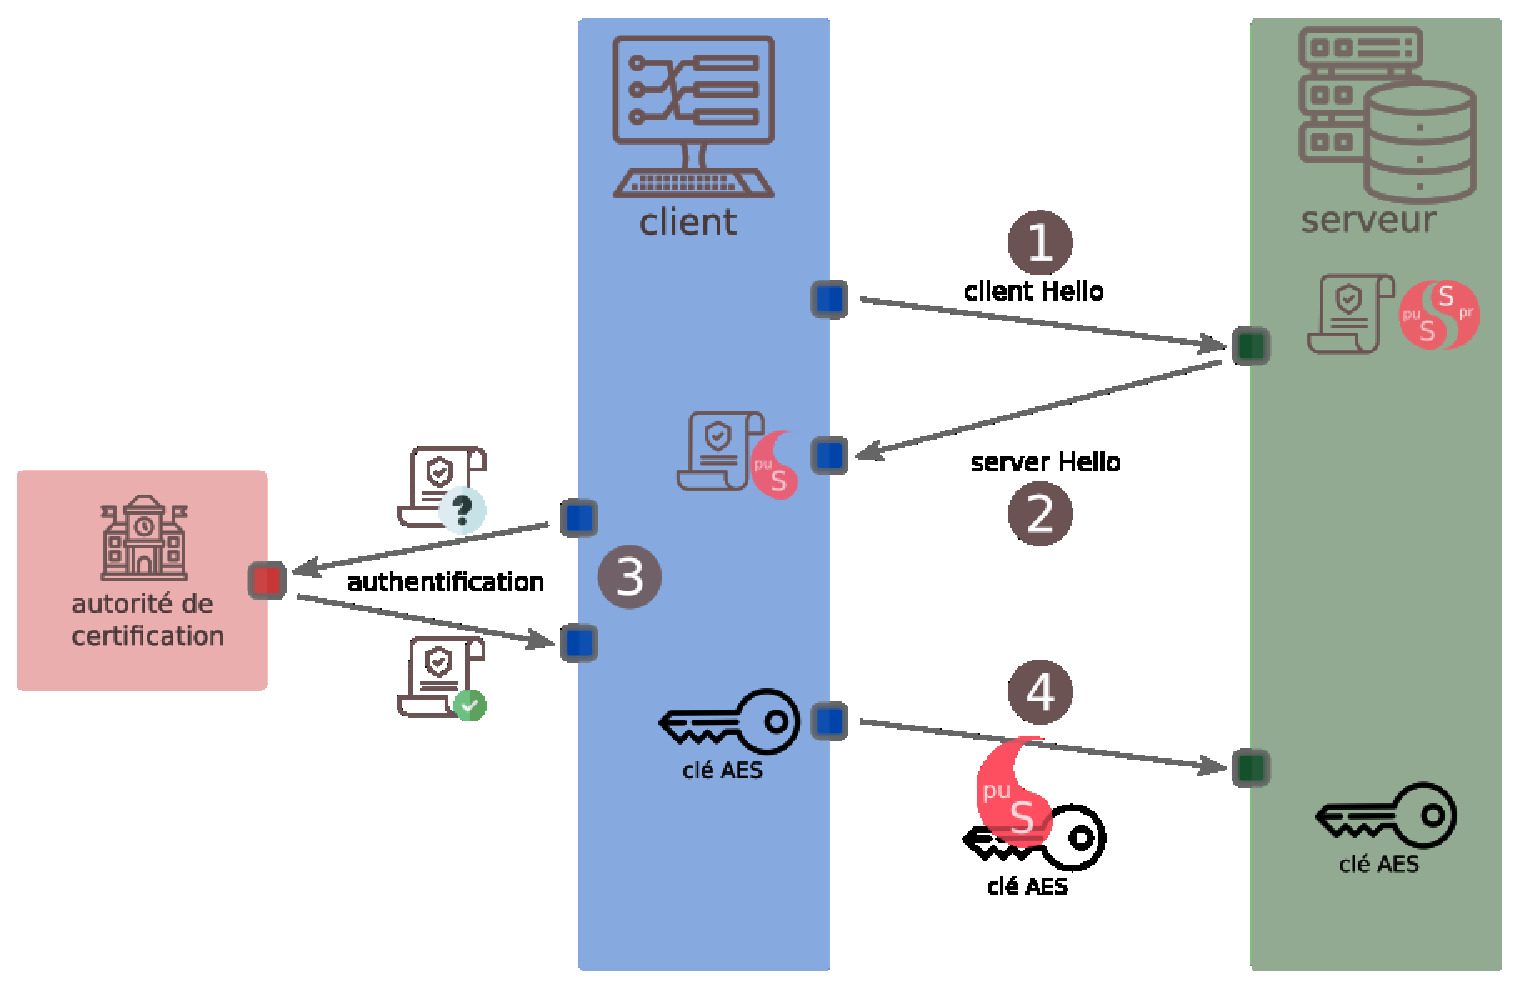
\includegraphics[height=160px]{tls.eps}
		\end{center}
	\end{block}
\end{frame}

\end{document}